\documentclass[dvipdfmx]{beamer}
%\documentclass[dvipdfmx,handout]{beamer}

\usepackage{bxdpx-beamer}
\usepackage{pxjahyper}
\usepackage{minijs}
\usepackage{comment}
\usepackage{color}
\renewcommand{\kanjifamilydefault}{\gtdefault}
\renewcommand{\figurename}{図}
\renewcommand{\tablename}{表}

\AtBeginDvi{\special{pdf:tounicode 90ms-RKSJ-UCS2}}

\setbeamertemplate{navigation symbols}{}
\usetheme{Boadilla}
%\usecolortheme[RGB={30,30,137}]{structure}

\usefonttheme{professionalfonts}
\setbeamertemplate{theorems}[numbered]
\newtheorem{thm}{Theorem}[section]
\newtheorem{proposition}[thm]{Proposition}
\theoremstyle{example}
\newtheorem{exam}[thm]{Example}
\newtheorem{remark}[thm]{Remark}
\newtheorem{question}[thm]{Question}
\newtheorem{prob}[thm]{Problem}

\definecolor{ired}{rgb}{0.72, 0.33, 0.31}
\definecolor{iblue}{rgb}{0.42, 0.56, 0.75}

\setbeamertemplate{itemize item}{$\vartriangleright$}
\setbeamertemplate{itemize subitem}{$\blacktriangleright$}
\setbeamertemplate{itemize subsubitem}{$\blacktriangleright$}
\setbeamertemplate{enumerate item}[circle]

\begin{document}

\title[sample]{sample slide}
\institute[sugoi]{sugoiとこ}
\author[dokaraya]{$	\bigcirc$dokaraya}
\date{\today}

\begin{frame}
\titlepage
\nocite{*}
\end{frame}

\begin{frame}{目的}
  \begin{block}{目的}
    \begin{itemize}
      \item テンプレを置く.
    \end{itemize}
  \end{block}

  \begin{columns}[t]
  \begin{column}{0.55\textwidth}
    \begin{figure}
      \centering
      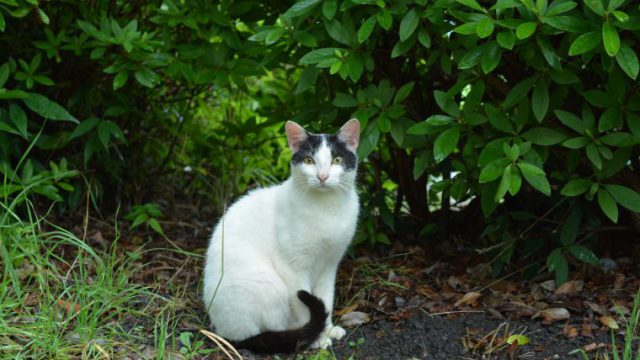
\includegraphics[width=5cm]{fig/img.jpg}
      \caption{素晴らしき猫}
      \label{fig:cat}
    \end{figure}
  \end{column}
  \begin{column}{0.45\textwidth}
    \begin{table}[t]
      \caption{かわいさ投票の結果}
      \label{tab:example}
      \centering
      \begin{tabular}{cr}
        \hline
        種類 & かわいさ(票)\\ \hline
        犬 & 100\\
        猫 & 100\\ \hline
        総数 & 200 \\ \hline
      \end{tabular}
    \end{table}
  \end{column}
\end{columns}
\end{frame}

\begin{frame}[allowframebreaks]{参考文献}
    \scriptsize
    \beamertemplatetextbibitems
    \bibliographystyle{junsrt}
    \bibliography{ref}
\end{frame}

\end{document}
